\section{Branch and Bound} \label{sec:branch-and-bound}

O método de Ramificar e limitar é uma forma de 
encontrar soluções ótimas para vários problemas de otimização, especialmente em 
otimização combinatória. Consiste em uma enumeração sistemática de todos os candidatos
a solução, através da qual grandes subconjuntos de candidatos infrutíferos são 
descartados em massa utilizando os limites superior e inferior da quantia otimizada.

O método foi proposto por A. H. Land e A. G. Doig em 1960 para programação discreta.
É utilizado para vários problemas NP-completos como o problema do caixeiro viajante
e o problema da mochila. 

\subsection{Problema da mochila}

\begin{figure}[ht]
    \centering
    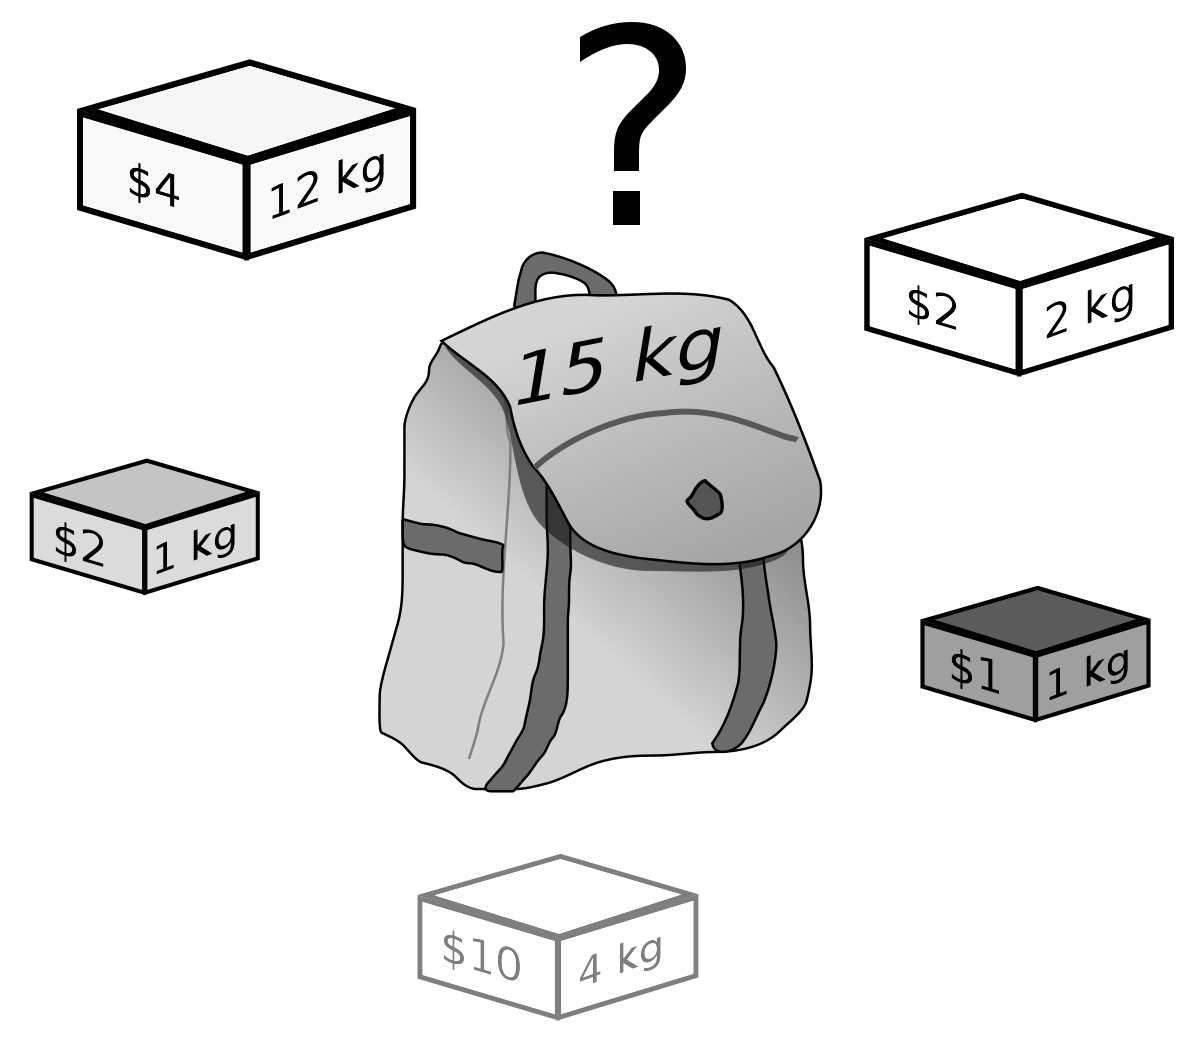
\includegraphics[width=.5\textwidth]{knapsack.png}
    \caption{Ilustração do problema da mochila}
    \label{fig:knapsack}
\end{figure}

\begin{algorithm}
    \caption{Knapsack}
    \begin{algorithmic}[1]
    \Procedure{knapsack}{}
    \State {$\text{colors} \gets \text{[G.vertex]}$}
    \For{$\text{v in G.V}$}
    \If{$\text{colors[v] == WHITE}$}
    \State {$\textbf{visit(v,colors)}$}
    \EndIf
    \EndFor
    \EndProcedure
    \Procedure{visit}{index,colors}
    \State {$\text{colors[index]} \gets \text{YELLOW}$}
    \For{$\text{v in G.adj[index]}$}
    \If{$\text{colors[v] == WHITE}$}
    \State {$\textbf{visit(v,colors)}$}
    \EndIf
    \EndFor
    \State {$\text{colors[index]} \gets \text{RED}$}
    \EndProcedure
    \end{algorithmic}
  \end{algorithm}

  \nocite{branch-and-bound}
  \nocite{knapsacker}

  \newpage